\section{The Area of Work}
 
\subsection{What is Big Data\& Why it matters}
Big data is an evolving term that describes any voluminous amount of structured, semi-structured and unstructured data that has the potential to be mined for information. Although big data doesn't refer to any specific quantity, the term is often used when speaking about petabytes and exabytes of data.

Big data can be characterized by 3Vs: the extreme volume of data, the wide variety of types of data and the velocity at which the data must be must processed.

\textbf{Volume} Big data implies enormous volumes of data. It used to be employees created data. Now that data is generated by machines, networks and human interaction on systems like social media the volume of data to be analyzed is massive \textbf{Variety}. Variety refers to the many sources and types of data both structured and unstructured. We used to store data from sources like spreadsheets and databases. Now data comes in the form of emails, photos, videos, monitoring devices, PDFs, audio, etc. This variety of unstructured data creates problems for storage, mining and analyzing data \textbf{Velocity}.    

Big Data Velocity deals with the pace at which data flows in from sources like business processes, machines, networks and human interaction with things like social media sites, mobile devices, etc. The flow of data is massive and continuous. This real-time data can help researchers and businesses make valuable decisions that provide strategic competitive advantages and ROI if you are able to handle the velocity.


\begin{figure}[htp]
\centering
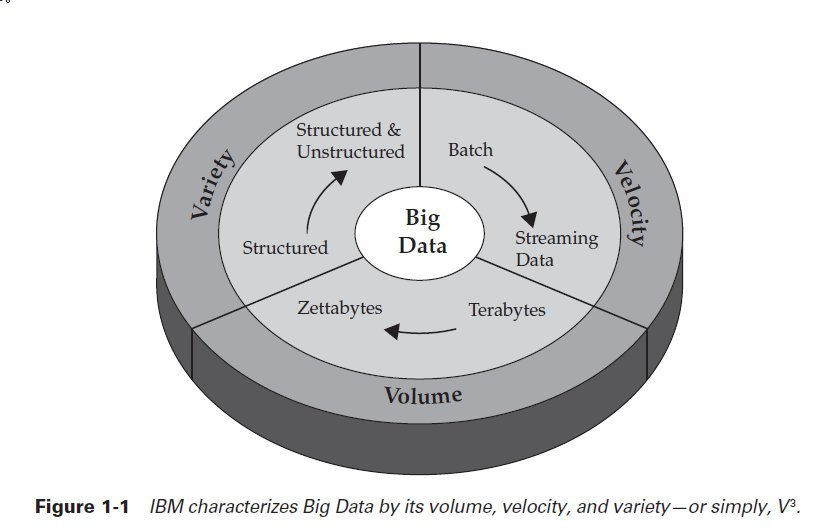
\includegraphics[scale=0.3]{Figures/fig-4.jpg}
\caption{}
\label{}
\end{figure}
A number of recent technology advancements enable organizations to make the most of big data and big data analytics:
\vspace*{-2mm}

\begin{description}
\vspace*{-2mm}
\item[1]Cheap, abundant storage.
\vspace*{-2mm}
\item[2]Faster processors.
\vspace*{-2mm}
\item[3]Affordable open source, distributed big data platforms, such as Hadoop.
\end{description}

\subsection{Hadoop}\cite{hadoop}
Apache Hadoop is an open source framework written in java for distributed storage and distributed processing of very large data sets on computer clusters built on commodity hardware. It is software framework for storing and processing big data.  It accomplishes two tasks massive data storage and faster processing.  Hadoop was initially inspired by papers published by Google outlining its approach to handling an avalanche of data, and has since become the de facto standard for storing,    processing and analyzing hundreds of terabytes, and even petabytes of data.  

Instead of relying on expensive, proprietary hardware and different systems to store and process data, Hadoop enables distributed parallel processing of huge amounts of data across inexpensive, industry-standard servers that both store and process the data, and can scale without limits. With Hadoop no data is considered to be big .It is designed up from a single server to thousands of machines. Rather than relying on high-end hardware, the resiliency of these clusters comes from the software's ability to detect and handle failures at the application layer.  And in today’s world where lots of amount of data is being created everyday , Hadoop’s breakthrough advantages mean that businesses and organizations can now find value in data that was recently considered useless. All the modules in hadoop are designed with a hardware  (of individual machines, or racks of machines) are commonplace and thus should be automatically handled in software by the framework.

The core of Apache hadoop consists of a Storage part HDFS(Hadoop Distributed File System) and has a processing part ( Map Reduce) .  Hadoop splits files into large blocks and distributes them amongst the nodes in the cluster. To process the large amount of data hadoop MapReduce transfer codes in the form package to nodes for the parallel processing  based on the data each node needs to process. This approach takes in account of data locality to manipulate the data on hand to allow the data to beprocessed faster and more efficiently than it would be in a more conventional supercomputer architecture that relies on a parallel file system where computation and data are connected via high-speed networking. The Apache hadoop software  library itself is designed to detect and handle failures at the application layer, so delivering a highly-available service on top of a cluster of computers, each of which may be prone to failures.

The Project includes these modules:
\begin{description}
\item[1. Hadoop Common]:  The common utilities that support the other Hadoop modules i.e  the requirements by the other modules.
\item[2. Hadoop Distributed File System (HDFS)]: It is a distributed file system that stores huge amount of data on commodity machines. A distributed file system that provides  high-throughput access to application data.
\item[3.Hadoop YARN]: It is a resource management platform i.e. a framework for job scheduling and cluster resource management.
\item[4. Hadoop MapReduce]: A YARN-based system for parallel processing of large data sets.

\end{description}
Hadoop was created by Doug Cutting, the creator of Apache Lucene, the widely used text search library. Hadoop has its origins in Apache Nutch, an open source web search engine, itself a part of the Lucene project.
Nutch was started in 2002, and a working crawler and search system quickly emerged. However their architecture wouldn’t scale to the billions of pages on the Web. In 2003 Google published paper on Google’s Distributed Filesystem (GFS) which was being used in production at Google. Hence in 2004 they implemented Nutch Distributed Filesystem  (NDFS) using GFS architecture that would solve their storage needs for very large files generated as a part of the web crawl and indexing process.
In 2004, Google published the paper that introduced MapReduce to the world. NDFS and the MapReduce implementation in Nutch were applicable beyond the realm of search, and in February 2006 they moved out of Nutch to form an independent subproject of Lucene called Hadoop.

\subsubsection{Why use Hadoop?}
Hadoop changes the economics and dynamic scale of large scale computing.
There are following characteristics of Hadoop.
\begin{description}

\item[1. Scalable] A cluster can be expanded by adding new servers or resources without having to move, reformat, or change the dependent analytic workflows or applications.
\item[2. Flexible] Hadoop is schema-less and can absorb any type of data,structured   or not, from any number of sources. Data from multiple sources can be joined and   aggregated in arbitrary ways enabling deeper analyses than any one system can provide i.e different data set can be combined of different formats to give a efficient result.
\item[3. Cost effective] Hadoop brings massively parallel computing to commodity servers. The result is a sizeable decrease in the cost per terabyte of storage, which in turn makes it affordable to model all your data.
\item[4. Fault tolerant]  When you lose a node, the system redirects work to another location of the data and continues processing without missing a beat.
\item[5. Massive storage]. The Hadoop framework can store huge amounts of data by breaking the data into blocks and storing it on clusters of lower-cost commodity hardware.
\item[6. Distributed] Data is divided and stored across multiple computers, and computations can be run in parallel across multiple connected machines.
i.e. collection of large datasets which allows to find out useful information.
\end{description}

\subsubsection{Hadoop Ecosystem}
Hadoop is supplemented by an ecosystem of Apache open-source projects that extend the value of Hadoop and improve its usability. Some of these Apache opensource software projects are: 
\begin{description}

\item[1. Pig]A programming language designed to handle any type of data, helping users to focus more on analyzing large data sets and less on writing map programs and reduce programs. 
\item[2. Hive]A Hadoop runtime component that allows those fluent with SQL to write Hive Query Language (HQL) statements, which are similar to SQL statements. These are broken down into MapReduce jobs and executed across the cluster.
\item[3. Flume]A distributed, reliable and available service for efficiently collecting, aggregating and moving large amounts of log data. Its main goal is to deliver data from applications to the HDFS. 
\item[4. HBase]A column-oriented non-relational (noSQL) database that runs on top of HDFS and is often used for sparse data sets. 
\item[5. Mahout]A Scalable machine learning and data mining library.
\item[6. Spark]A fast and general compute engine for Hadoop data. Spark provides a simple and expressive programming model that supports a wide range of applications, including ETL, machine learning, stream processing, and graph computation.
\item[7. Cassandra]A scalable multi-master database with no single points of failure.
\end{description}

\subsubsection{Hadoop Architecture}
Hadoop consists of the Hadoop common package which provides file system and OS level architecture a map reduce engine and a Hadoop distributed file system (HDFS) . The Hadoop Common package contains the necessary Java ARchive (JAR) files and scripts needed to start Hadoop.  

For effective scheduling of the work , every Hadoop compatible file system should provide location awareness the name of the rack where work node is located. The goal is to reduce the impact of a rack power outage or switch failure, so that even if these events occur, the data may still be readable. A small Hadoop cluster has a single master node and multiple worker nodes. The master node includes  a Job Tracker , Task Tracker, Name Node and Data Node. 

A slave or worker node behaves as both a Data Node and Task Tracker, though it is possible to have data-only worker nodes and compute-only worker nodes. These are normally used only in nonstandard applications. Hadoop requirement is Java Runtime Environment  version 1.6 or higher. In a large cluster of data HDFS is controlled by Name Node server to host the file system index, and a secondary Name Node that can generate snapshots of the name node's memory structures. It  prevents file-system corruption and reduces loss of data. Job tracker server manages scheduling of jobs in a server. In cluster Hadoop map reduce engine is being used against an alternating file system the name node, secondary name node, data node architecture of HDFS are updated by file system Specific equivalent.

\subsection{MapReduce}
MapReduce is a programming paradigm for easily writing applications which process vast amounts of data (multi-terabyte data-sets) in-parallel on large clusters (thousands of nodes) of commodity hardware in a reliable, fault-tolerant manner. The framework is divided into two parts: Map, allows to parcels out work to different nodes in the distributed cluster. Reduce, collates the work and resolves the results into a single value.

MapReduce framework consists of a single master JobTracker and one slave TaskTracker per cluster-node. Master is responsible for scheduling the jobs' component tasks on the slaves, monitoring them and re-executing the failed tasks. Although the Hadoop framework is implemented in Java, MapReduce applications can be written in Python, Ruby, R, C++. Eg. Hadoop Streaming, Hadoop Pipes.

\subsubsection{Hadoop-MapReduce Architecture}
\begin{figure}[htp]
\centering
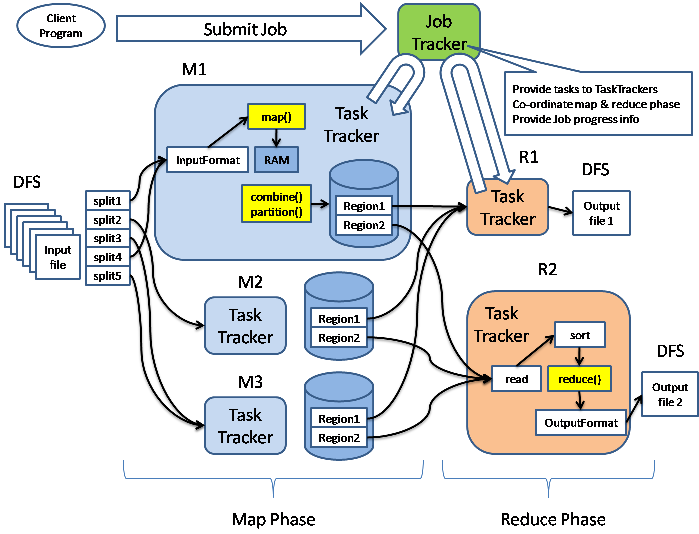
\includegraphics[scale=0.7]{Figures/fig-5.png}
\caption{}
\label{}
\end{figure}
Hadoop MapReduce is a software framework for easily writing applications which process vast amounts of data (multi-terabyte data-sets) in-parallel on large clusters (thousands of nodes) of commodity hardware in a reliable, fault-tolerant manner.
A MapReduce job usually splits the input data-set into independent chunks which are processed by the map tasks in a completely parallel manner. The framework sorts the outputs of the maps, which are then input to the reduce tasks. Typically both the input and the output of the job are stored in a file-system. The framework takes care of scheduling tasks, monitoring them and re-executes the failed tasks.
The MapReduce framework consists of a single master JobTracker and one slave TaskTracker per cluster-node. The master is responsible for scheduling the jobs' component tasks on the slaves, monitoring them and re-executing the failed tasks. The slaves execute the tasks as directed by the master.
The MapReduce framework operates exclusively on <key, value> pairs, that is, the framework views the input to the job as a set of <key, value> pairs and produces a set of <key, value> pairs as the output of the job, conceivably of different types.
\begin{description}
\item[Map]: Each worker node applies the "map()" function to the local data, and writes the output to a temporary storage. A master node arrange that for redundant copies of input data, only one is processed.

\item[Shuffle]: Worker nodes redistribute data based on the output keys (produced by the "map()" function), such that all data belonging to one key is located on the same worker node.
\item[Reduce]: Worker nodes now process each group of output data, per key, in parallel.
\end{description}

\begin{figure}[htp]
\centering
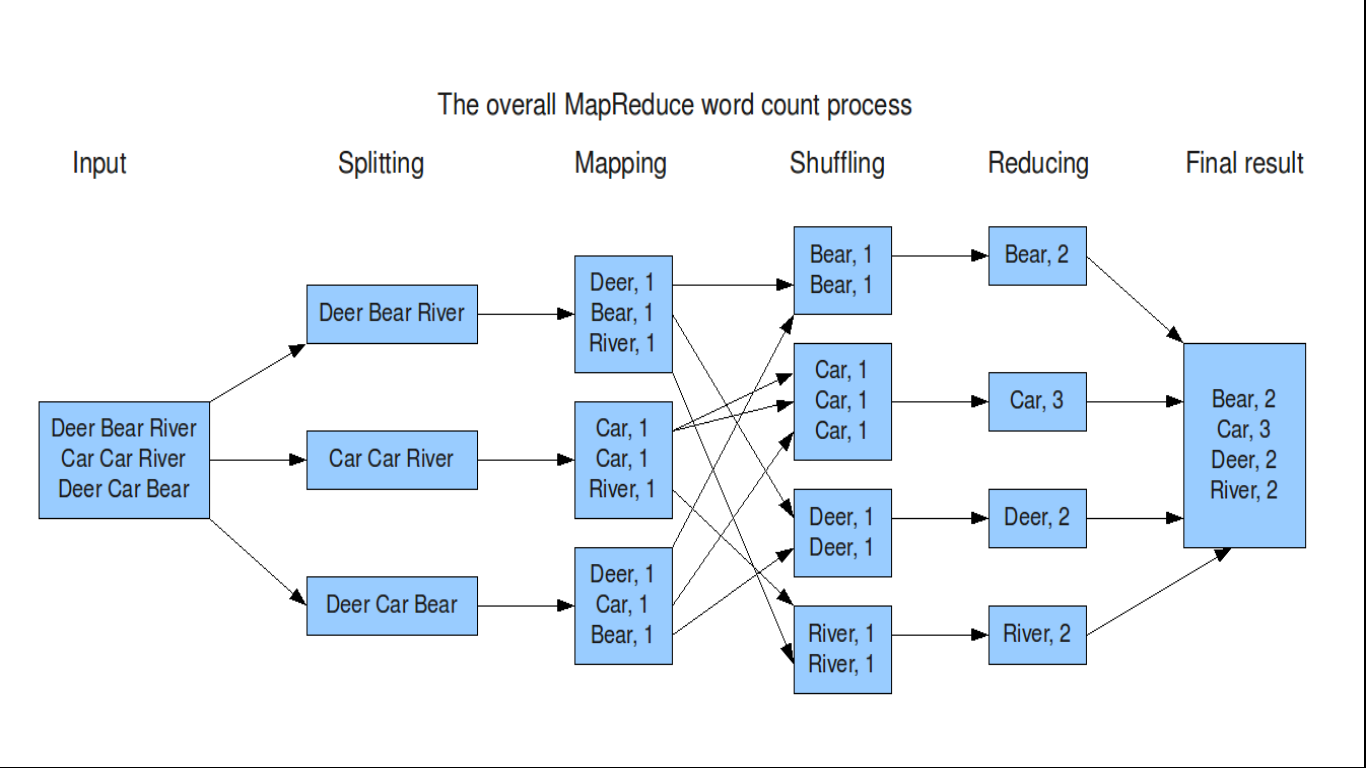
\includegraphics[scale=0.3]{Figures/fig-6.png}
\caption{}
\label{}
\end{figure}

\subsubsection{Map Reduce in Amazon Aws EC2} Amazon Elastic MapReduce (Amazon EMR) is a web service that makes it easy to quickly and cost-effectively process vast amounts of data. Amazon Elastic MapReduce (Amazon EMR) is a web service that makes it easy to quickly and cost-effectively process vast amounts of data.
Amazon EMR simplifies big data processing, providing a managed Hadoop framework that makes it easy, fast, and cost-effective for you to distribute and process vast amounts of your data across dynamically scalable Amazon EC2 instances. The EC2 instances used to run an Elastic MapReduce job flow fall in to one of three categories or instance groups:
\begin{description}
\item[Master]The Master instance group contains a single EC2 instance. This instance schedules Hadoop tasks on the Core and Task nodes.
\item[Core]The Core instance group contains one or more EC2 instances. These instances use HDFS to store the data for the job flow. They also run mapper and reducer tasks as specified in the job flow. This group can be expanded in order to accelerate a running job flow.
\item[Task]The Task instance group contains zero or more EC2 instances and runs mapper and reduce tasks. Since they don’t store any data, this group can expand or contract during the course of a job flow.
\end{description}

\subsubsection{MapReduce MapR}
MapR is a third-party application offering an open, enterprise-grade distribution that makes Hadoop easier to use and more dependable. For ease of use, MapR provides network file system (NFS) and open database connectivity (ODBC) interfaces, a comprehensive management suite, and automatic compression. For dependability, MapR provides high availability with a self-healing no-NameNode architecture, and data protection with snapshots, disaster recovery, and with cross-cluster mirroring.

All three MapR Editions for Hadoop (M7, M5 and M3) are available within the EMR service.
MapR M7 is the fastest and most reliable distribution for Apache Hadoop, and includes an enterprise-grade online database that adds the speed, scalability, and flexibility of NoSQL databases. MapR M7 is the only distribution built for running both operational and analytical workloads in the same cluster.

\subsection{Hadoop Distributions}
These products have been emerged out from Hadoop and incresingly become fast, reliable and scalable.

\subsubsection{Cloudera Hadoop}
Cloudera Inc. was founded by big data geniuses from Facebook, Google, Oracle and Yahoo in 2008. It was the first company to develop and distribute Apache Hadoop-based software and still has the largest user base with most number of clients. Although the core of the distribution is based on Apache Hadoop, it also provides a proprietary Cloudera Management Suite to automate the installation process and provide other services to enhance convenience of users which include reducing deployment time, displaying real time nodes’ count, etc.

\subsubsection{Hortonworks Hadoop}
Hortonworks, founded in 2011, has quickly emerged as one of the leading vendors of Hadoop. The distribution provides open source platform based on Apache Hadoop for analysing, storing and managing big data. Hortonworks is the only commercial vendor to distribute complete open source Apache Hadoop without additional proprietary software. Hortonworks’ distribution HDP2.0 can be directly downloaded from their website free of cost and is easy to install. The engineers of Hortonworks are behind most of Hadoop’s recent innovations including Yarn, which is better than MapReduce in the sense that it will enable inclusion of more data processing frameworks.

\subsubsection{Apache Spark}
Unlike Hadoop which is a batch processing system, it provides Real-Time Analytics.
\begin{description}
\item[1. Fast Analytics and Stream Processing] Apache Spark is an open source, parallel data processing framework that complements Apache Hadoop to make it easy to develop fast, unified Big Data applications combining batch, streaming, and interactive analytics on all your data

\item[2. Fast, Powerful Data Processing] For analysts and data scientists who rely on iterative algorithms (e.g. clustering/classification), Spark is 10-100x faster than MapReduce delivering faster time to insight on more data, resulting in better business decisions and user outcomes. Spark is 
\begin{description}
\item[Fast]: Data processing up to 100x faster than MapReduce, both in-memory and on disk
\item[Powerful]: Write sophisticated parallel applications quickly in Java, Scala, or Python without having to think in terms of only “map” and “reduce” operators
\item[Integrated]: Spark is deeply integrated with CDH, able to read any data in HDFS and deployed through Cloudera Manager
\end{description}
\end{description}

\subsection{Data Analytics and Visualization}
Data analytics (DA) is the science of examining raw data with the purpose of drawing conclusions about that information. Data analytics is used in many industries to allow companies and organization to make better business decisions and in the sciences to verify or disprove existing models or theories. Data analytics is distinguished from data mining by the scope, purpose and focus of the analysis. Data miners sort through huge data sets using sophisticated software to identify undiscovered patterns and establish hidden relationships. Data analytics focuses on inference, the process of deriving a conclusion based solely on what is already known by the researcher.

Data visualization is the presentation of data in a pictorial or graphical format. For centuries, people have depended on visual representations such as charts and maps to understand information more easily and quickly.

As more and more data is collected and analyzed, decision makers at all levels welcome data visualization software that enables them to see analytical results presented visually, find relevance among the millions of variables, communicate concepts and hypotheses to others, and even predict the future.

Because of the way the human brain processes information, it is faster for people to grasp the meaning of many data points when they are displayed in charts and graphs rather than poring over piles of spreadsheets or reading pages and pages of reports.

Interactive data visualization goes a step further – moving beyond the display of static graphics and spreadsheets to using computers and mobile devices to drill down into charts and graphs for more details, and interactively (and immediately) changing what data you see and how it is processed.

\subsubsection{Tools for Data Visualization}
There are abundant visulization tools but most widely used opensource tools are:
\begin{description}
\item[ggplot] ggplot2 is a plotting system for R, based on the grammar of graphics, which tries to take the good parts of base and lattice graphics and none of the bad parts. It takes care of many of the fiddly details that make plotting a hassle (like drawing legends) as well as providing a powerful model of graphics that makes it easy to produce complex multi-layered graphics.
\item[googleVis] googleVis is an R package providing an interface between R and Google Charts. The functions of the package allow the user to visualise data with the Google Chart Tools without uploading their data to Google. The output of googleVis functions is html code that contains the data and references to JavaScript functions hosted by Google. To view the output a browser with Flash and Internet connection is required, the actual chart is rendered in the browser. 
\item[D3] D3 allows you to bind arbitrary data to a Document Object Model (DOM), and then apply data-driven transformations to the document. For example, you can use D3 to generate an HTML table from an array of numbers. Or, use the same data to create an interactive SVG bar chart with smooth transitions and interaction. 
\end{description}
\section{Problem Addressed}
Aviation and air travel has established itself as a key economic and social resource in modern times. As the world population increases and becomes ever more interconnected, the demand for air travel will only increase. Currently there are over 100,000 commercial aviation flights and over 200,000 general aviation flights within the national airspace system (NAS) every day. This does not include military sorties or other, special purpose, flights within the NAS. The number of passengers flying to or from the U.S. is expected to grow an
average of 4.5\% annually, with cargo amounts showing a similar increase, while general aviation is expected to
grow 1\% annually. In addition, there is increasing interest, from both government and commercial sectors, in integrating unmanned aerial vehicles (UAV’s) into the NAS. Though full UAV integration poses its own unique set of complications, nevertheless it is only a matter of time before they contribute to the air traffic over the NAS. This constant increase in air traffic within the increasingly congested NAS will require new methods and techniques to efficiently accommodate new traffic.

To address these issues, the US Congress approved plans for the development of the Next Generation Air Transportation System (NextGen). It is an overhaul of the current NAS with the goals of allowing more aircraft to safely fly closer together with more direct
routes. It is scheduled for implementation in stages between 2012 and 2025 with 5 major elements: (i) Automatic dependent surveillance-broadcast (ADS-B) will replace radar systems with satellite based global positioning information for each aircraft. This infor- mation will be broadcast in realtime to airports another aircraft within a 150 mile radius allowing them to fly closer without jeopardizing safety. (ii) Systemwide information management (SWIM) is a consolidation of multiple information systems into a single coherent system and will reduce redundancy and facilitate information sharing. (iii) NextGen data communication will add data links between aircraft and air traffic controllers to the current two-way voice communication. (iv) NextGen network enabled weather is an ambitious effort to fuse data from tens of thousands of ground, air, and space based sensors into a single national weather information system to provide realtime weather information. (v) NAS voice switch (NVS) will replace multiple existing voice switching systems into a single consolidated air/ground and ground/ground voice communication system.The NextGen system will provide the infrastructure to allow aircraft to safely fly closer together thereby making more efficient use of limited airspace. It will allow aircraft to use more direct routes instead of being constrained to predetermined sky highways thereby
reducing congestion and reduce fuel costs. With pieces of the NextGen infrastructure coming into place, there is an opportunity to further their benefits by developing software tools that provide added value.

 This paper focuses on visual analysis tools to study the changes on air traffic congestion in span of 21 years which would allow policy makers to see the effects of changing the aircraft separation volume on congestion. The same tool can also be used as a decision aid for processing requests for unmanned aerial vehicle operations. Specifically, this paper will discuss methods
and tools used to calculate and render air traffic densities over areas of interest, as well as methods for aggregating such traffic densities over different time scales to extract fluctuations and periodic cycles in traffic patterns. We apply these tools to study the effects of possible modifications to the current en-route aircraft separation requirements. These modification, which are based on the characteristics of large fixed wing aircraft, has the potential of increasing the amount of available air space, allowing for future increases in overall air traffic numbers. In addition, we apply the same suite of tools to provide a quick visual inspection of planned UAV operation under different aircraft separation requirements. The studies conducted in this paper are based on a data set which is constructed from information made available by the Bureau of Transportation Statistics, 

There are over 300,000 flightswithin the United States every day. In the future, daily air traffic number of all varieties are expected to continue rising. In addition, there is increasing interest in integrating unmanned aerial vehicles, for both government and commercial interests, into the national airspace system (NAS). This large growth in aviation operations will only increase traffic within the already limited NAS, leading to higher congestion and less free airspace. In this report, we present visual analysis tools
to study the changes on air traffic congestion in span of 21 years. The tools support visualization of time-varying
air traffic density over an area of interest using different time granularity. We use this visual analysis
platform to investigate how changing the aircraft separation volume can reduce congestion while maintaining key safety requirements. The same tool can also be used as a decision aid for processing requests for unmanned aerial vehicle operations.

To present our analysis on traffic we utilized Airline Data presented at ASA Data Expo 2009. This dataset is constructed from information made available by the Bureau of Transportation Statistics, USA. It consists of more than 120 million records corresponding to each commercial airline flight in the United States between 1987 and 2008. As datasets gets larger, real-time visualization becomes more difficult. Supposedly a dataset with a billion entries. If we compute a summary of the dataset and visualize it we will either need non-trivial parallel rendering algorithms or significant time to produce a drawing. This solutions would not scale well. To perform analysis we need to mine relevant data using MapReduce programming. 
 

\subsection{Data}
The data comes originally from RITA where it is described in detail. It can download the data there, or from the bzipped csv files listed below. These files have derivable variables removed, are packaged in yearly chunks and have been more heavily compressed than the originals.

\begin{tabular}{llll}
	Variable & Description & Variable & Description\\
	Year & 1987-2008 & DepDelay & departure delay, in minutes\\
	Month & 1-12 & Origin & 	origin IATA airport code\\
	DayofMonth & 1-31 & Dest & 	destination IATA airport code\\
	DayOfWeek & 1 (Monday) - 7 (Sunday) & Distance & in miles\\
	DepTime & actual departure time (local, hhmm) & TaxiIn & taxi in time, in minutes\\
	CRSDepTime & scheduled departure time (local, hhmm) & TaxiOut & taxi out time in minutes\\
	ArrTime & actual arrival time (local, hhmm) & Cancelled & was the flight cancelled?\\
	CRSArrTime  & scheduled arrival time (local, hhmm) & CancellationCode & 	reason for cancellation (A = carrier, B = weather, C = NAS, D = security)\\
	UniqueCarrier & 	unique carrier code & Diverted & 1 = yes, 0 = no\\
	FlightNum & flight number & CarrierDelay & in minutes\\
	TailNum & plane tail number & WeatherDelay & in minutes\\
	ActualElapsedTime  & in minutes & NASDelay & in minutes\\
	CRSElapsedTime &  	in minutes & SecurityDelay & in minutes\\
	AirTime & in minutes & LateAircraftDelay & in minutes\\
	ArrDelay & arrival delay, in minutes &  & \\
\end{tabular}






\subsection{Goal}
This is intentionally vague in order to allow different entries to focus on different aspects of the data, but here are a few ideas to that we focussed on :
\vspace*{-2mm}
\begin{description}
  \item[-] Summarize data by time periods, airport, and carrier

  \vspace*{-4mm}

  \item[-] Temporal effects
  \vspace*{-4mm}
  \begin{description}
  \item[-] Are some time periods more prone to delays than others?
  \vspace*{-3mm}
  \item[-] Relationships between delays and \textit{Seasonal factors}: winter, summer, holidays \textit{Weather factors}: Blizzards and severe weather \textit{Daily factors}: Time of day, day of week
  \end{description}
  \vspace*{-4mm}
  \item[-] Spatial effects
  \vspace*{-2mm}
  \begin{description}
  \item[-] Are some airports more prone to delays than others?
  \end{description}
  \vspace*{-2mm}
  \item[-] Carrier effects
  \begin{description}
    \vspace*{-2mm}
  \item[-] Are some carriers more prone to delays than others?
  \end{description}

  \vspace*{-4mm}
  \item[-] Analysis of traffic on New York and Chicago a densly populated metropolitan cities in USA?

\end{description}

\subsection{Tools Used} % (fold)
Rhipe packages are used for the development of the MapReduce modal. R is used for Visualization along with googleVis and Shiny app to make it interactive.

\subsubsection{R}
R is a programming language and software environment for statistical computing and graphics. The R language is widely used among statisticians and data miners for developing statistical software and data analysis.

\subsubsection{Rhipe}
RHIPE is an R package that provides a way to use Hadoop from R. It can be used on its own or as part of the Tessera environment. RHIPE (hree-pay') is the R and Hadoop Integrated Programming Environment. RHIPE is a merger of R and Hadoop. R is the widely used, highly acclaimed interactive language and environment for data analysis. Hadoop consists of the Hadoop Distributed File System (HDFS) and the MapReduce distributed compute engine. RHIPE allows an analyst to carry out D\&R analysis of complex big data wholly from within R. RHIPE communicates with Hadoop to carry out the big, parallel computations. 

\subsubsection{ggplot}
ggplot2 is a plotting system for R, based on the grammar of graphics, which tries to take the good parts of base and lattice graphics and none of the bad parts. It takes care of many of the fiddly details that make plotting a hassle (like drawing legends) as well as providing a powerful model of graphics that makes it easy to produce complex multi-layered graphics.







\section{Existing System}
The main thrust of this paper is on visual analysis of air traffic data. Hence, this section focuses on work related to visualizing air traffic data. One of the most popular technique for visualizing air traffic data is to represent the trajectory of each aircraft as an animated particle. Many such visualizations are available on the web via sites such as youtube. A version that was designed by Aaron Koblin demonstrates several techniques and embellishments for presenting the flight trajectories. More recently, the discrete nature of the flight tracks were smoothed out to obtain a continuous estimate of air traffic density using a view dependent kernel density estimator. Representing air traffic data as a density plot is not new. Kellner [8] also used density plots of the arrival and departure rates of aircraft at different airports to assess their capacity. This paper will use similar techniques in visualizing the air traffic data. More importantly, our work examines the impact of varying minimum aircraft separation policy on air traffic density, and also examines if a flight plan, e.g. of a UAV operation request, will endanger existing flight patterns.

There are many factors affecting air traffic congestion and airport capacity. One of those that is controllable and fall under policy decisions is the specification of minimum separation between aircraft. Currently, this is set to 5 nautical miles horizontally, and 1,000
feet vertically [4] when the aircraft is en-route. This limit is adjusted as the aircraft approaches an airport and can drop to 3 miles horizontally on landing approaches to airports. The relative weight class of the leading and following aircraft are also taken into con-
sideration in such situations in order to reduce risks due to wake turbulence [3]. The en-route limit accounts for aircraft speed (typical passenger jets fly at average speed of 500 miles per hour or just over 8 miles per minutes), weather impact on visibility, and wake turbulence from leading aircraft, among other factors. With the touted capabilities of ADS-B, the NextGen enabled weather system, and integrated information system, one can theoretically safely reduce the minimum separation requirements between aircraft. This paper provides visual analysis tools to examine the effects of different shapes and parameters describing the minimum separation volume between aircraft.

With regards to UAV operation, they are more generally referred to as Unmanned Aircraft Systems (UAS)[7, 2]. Over the past few years, interest in UAS has rapidly increased. This is because of the possibilities they offer to both government and commercial interests. They would enable a broad range of satellite-like abilities, but at a much lower cost. Aerial photography, communications, environmental monitoring, and security are some of the abilities that UAS deployment could make possible on a large scale. Currently, UAS are predominantly used by the Department of Defense and the Department of Homeland Security, and often outside of national air space (NAS). A handful of UAS are allowed to operate inside our NAS, though almost exclusively for national security or research purposes. However, each UAS operation must be pre-approved by the FAA on a case by case basis. This process is very tedious and does not scale well to large numbers of flights. There are a few studies on risk managment of operating UAS. A recent study uses a site-specific non- uniform probabilistic background air traffic to study the risks [11]. Using the visual analysis tools presented in this paper, checking whether the flight plan for a UAS will allow for a safe operation within the NAS can be accomplished expeditiously.


\subsection{The  Oracle Airline Data Model} 
The  Oracle  Airline Data Model is a powerful logical and physical data model that will help  airlines effectively store, manage, and analyze airline data that currently resides in passenger service systems (includes
reservation systems and departure control systems), global distribution system (GDS), loyalty management systems, and customer data warehouses.  It provides a single scalable repository for transactional and historical data 
that can be used to provide real-time business intelligence and strategic 
insights you’re  your airline. Using sophisticated trending and data mining capabilities based on Oracle’s  OLAP and data mining technology,  airline personnel will now have the data analysis  capabilities to develop Airline -specific insights that are relevant, actionable, and can improve both top-line and bottom-line results. 

The Oracle Airline Data Model provides detail transaction storage and advanced analysis into a full range of airline
subject areas, including reservations, sales, operations, loyalty, 
and finance.  Using reservation data, the data model can provide detailed insight into passenger bookings by time period, fare class, and flight.  It provides insights into channel performance looking at bookings, cancellations, and revenues through travel agency, OTA, ticket counter, call center, and web channels.  It allows you to analyze passenger 
revenues by geography, time period, and flight.  Finally it provides insights into loyalty program member activity through a variety of reports.  
The data model fits the needs of large network carriers and low-cost carriers. 

 





